\documentclass[12pt,letterpaper,oneside,titlepage]{article}
\usepackage[latin1]{inputenc}
\usepackage{amsmath}
\usepackage{amsfonts}
\usepackage{amssymb}
\usepackage{graphicx}
\usepackage[letterpaper, portrait, margin=.5in]{geometry}
\usepackage{lscape}
\usepackage{tikz}
\usepackage{color}
\usepackage{tabto}
\usepackage{pgfplots}



\begin{document}
\author{Scott \textbf{``Cash''} Fields}
\title{GRAPHS}

%%%%%   LEARN     %%%%%%%%%%%%%%%%%%%%%
%%%%%%%%%%%%%%%%%%%%%%%%%%%%%%%%
\pagebreak
\begin{center}
	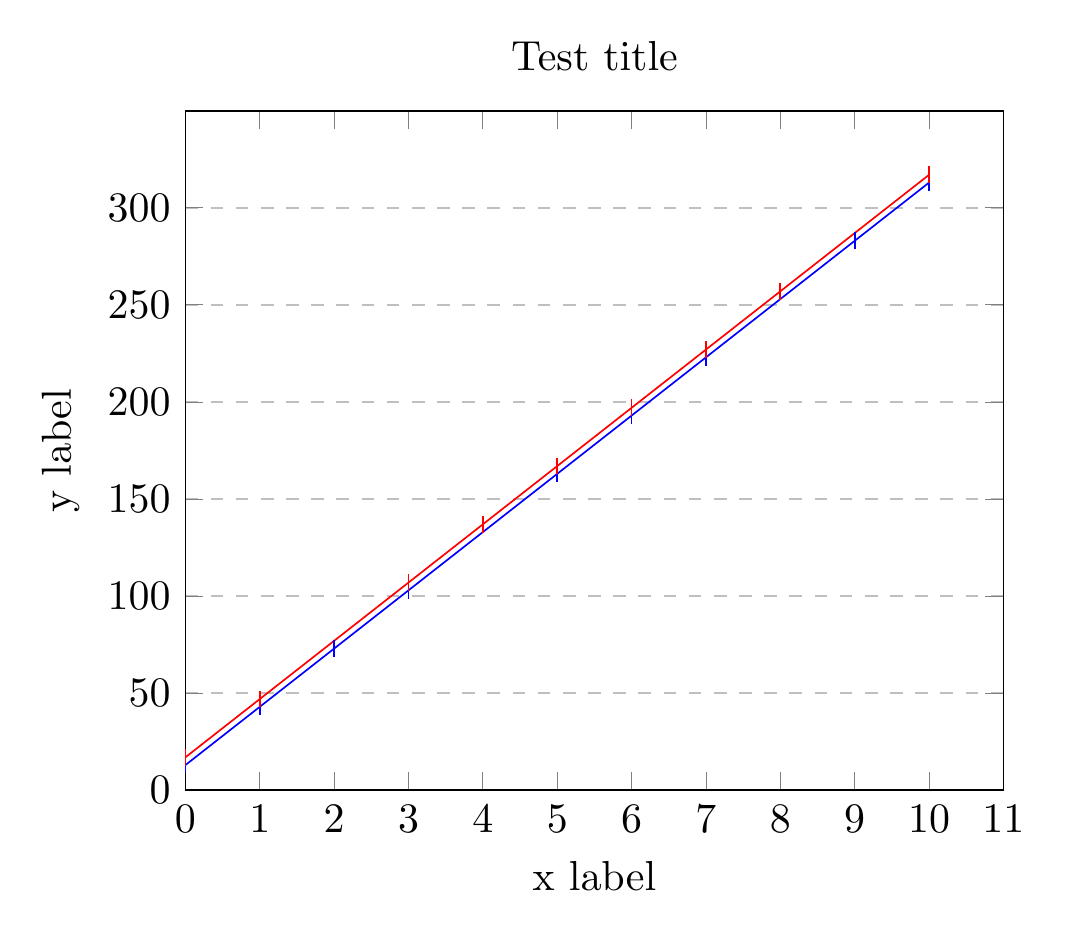
\begin{tikzpicture}[scale=\textwidth/8cm,]
	\begin{axis}[
	title={Test title},
	xlabel={x label},
	ylabel={y label},
	xmin=0, xmax=11,
	ymin=0, ymax=350,
	xtick={0,1,2,3,4,5,6,7,8,9,10,11},
	ytick={0,50,100,150,200,250,300},
	legend pos=north west,
	ymajorgrids=true,
%	xmajorgrids=true,
	grid style=dashed,
	]
	
	\addplot[
	color=blue,
	%dotted,
	mark=|,
	%mark options={solid},
	%smooth
	%%mark=dot,
	]
	coordinates {
		%%      (0,23.1)(10,27.5)(20,32)(30,37.8)(40,44.6)(60,61.8)(80,83.8)(100,114)
		(000,13)
		(001,43)
		(002,73)
		(003,103)
		(005,163)
		(006,193)
		(007,223)
		(009,283)
		(010,313)
		%(012,373)
		%(014,433)
		%(015,463)
		%(017,523)
		%(020,613)
		%(021,643)
		%(022,673)
		%(024,733)
		%(027,823)
		%(028,853)
		%(029,883)
		%(034,1033)
		%(035,1063)
		%(036,1093)
		%(037,1123)
		%(038,1153)
		%(040,1213)
		%(043,1303)
		%(047,1423)
		%(048,1453)
		%(049,1483)
		%(051,1543)
		%(055,1663)
		%(056,1693)
		%(057,1723)
		%(058,1753)
		%(059,1783)
		%(062,1873)
		%(064,1933)
		%(066,1993)
		%(068,2053)
		%(069,2083)
		%(070,2113)
		%(071,2143)
		%(073,2203)
		%(076,2293)
		%(079,2383)
		%(082,2473)
		%(083,2503)
		%(086,2593)
		%(089,2683)
		%(090,2713)
		%(093,2803)
		%(094,2833)
		%(098,2953)
	};
	\addplot[
	color=red,
	%dotted,
	mark=|,
	%mark options={solid},
	%smooth
	%%mark=dot,
	]
	coordinates {
		(000,17)
		(001,47)
		(003,107)
		(004,137)
		(005,167)
		(006,197)
		(007,227)
		(008,257)
		(010,317)
		%(011,347)
		%(015,467)
		%(018,557)
		%(019,587)
		%(020,617)
		%(021,647)
		%(022,677)
		%(026,797)
		%(027,827)
		%(028,857)
		%(029,887)
		%(031,947)
		%(032,977)
		%(036,1097)
		%(039,1187)
		%(040,1217)
		%(042,1277)
		%(043,1307)
		%(045,1367)
		%(047,1427)
		%(049,1487)
		%(053,1607)
		%(054,1637)
		%(055,1667)
		%(056,1697)
		%(059,1787)
		%(061,1847)
		%(062,1877)
		%(063,1907)
		%(066,1997)
		%(067,2027)
		%(069,2087)
		%(073,2207)
		%(074,2237)
		%(075,2267)
		%(076,2297)
		%(078,2357)
		%(080,2417)
		%(081,2447)
		%(082,2477)
		%(088,2657)
		%(089,2687)
		%(092,2777)
		%(094,2837)
		%(096,2897)
		%(097,2927)
		%(098,2957)
	};
	%\legend{CuSO$_4\cdot$5H$_2$O}
\end{axis}
\end{tikzpicture}
\end{center}

\pagebreak
\pagebreak
\begin{center}
	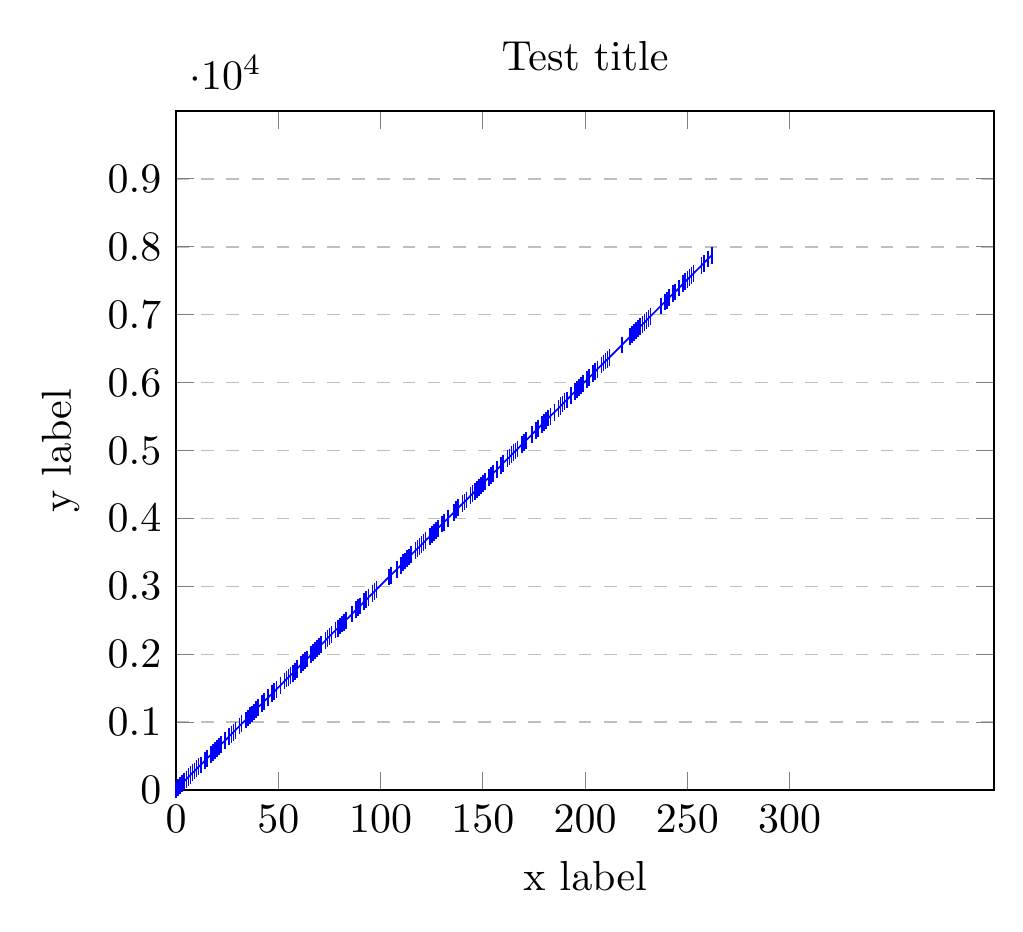
\begin{tikzpicture}[scale=\textwidth/8cm,]
\begin{axis}[
title={Test title},
xlabel={x label},
ylabel={y label},
xmin=0, xmax=400,
ymin=0, ymax=10000,
xtick={0,50,100,150,200,250,300},
ytick={0,1000,2000,3000,4000,5000,6000,7000,8000,9000},
legend pos=north west,
ymajorgrids=true,
grid style=dashed,
]

\addplot[
color=blue,
mark=|,
]
coordinates {
	(000,13)
	(000,17)
	(001,43)
	(001,47)
	(002,73)
	(003,103)
	(003,107)
	(004,137)
	(005,163)
	(005,167)
	(006,193)
	(006,197)
	(007,223)
	(007,227)
	(008,257)
	(009,283)
	(010,313)
	(010,317)
	(011,347)
	(012,373)
	(014,433)
	(015,463)
	(015,467)
	(017,523)
	(018,557)
	(019,587)
	(020,613)
	(020,617)
	(021,643)
	(021,647)
	(022,673)
	(022,677)
	(024,733)
	(026,797)
	(027,823)
	(027,827)
	(028,853)
	(028,857)
	(029,883)
	(029,887)
	(031,947)
	(032,977)
	(034,1033)
	(035,1063)
	(036,1093)
	(036,1097)
	(037,1123)
	(038,1153)
	(039,1187)
	(040,1213)
	(040,1217)
	(042,1277)
	(043,1303)
	(043,1307)
	(045,1367)
	(047,1423)
	(047,1427)
	(048,1453)
	(049,1483)
	(049,1487)
	(051,1543)
	(053,1607)
	(054,1637)
	(055,1663)
	(055,1667)
	(056,1693)
	(056,1697)
	(057,1723)
	(058,1753)
	(059,1783)
	(059,1787)
	(061,1847)
	(062,1873)
	(062,1877)
	(063,1907)
	(064,1933)
	(066,1993)
	(066,1997)
	(067,2027)
	(068,2053)
	(069,2083)
	(069,2087)
	(070,2113)
	(071,2143)
	(073,2203)
	(073,2207)
	(074,2237)
	(075,2267)
	(076,2293)
	(076,2297)
	(078,2357)
	(079,2383)
	(080,2417)
	(081,2447)
	(082,2473)
	(082,2477)
	(083,2503)
	(086,2593)
	(088,2657)
	(089,2683)
	(089,2687)
	(090,2713)
	(092,2777)
	(093,2803)
	(094,2833)
	(094,2837)
	(096,2897)
	(097,2927)
	(098,2953)
	(098,2957)
	(104,3137)
	(105,3163)
	(105,3167)
	(108,3253)
	(108,3257)
	(110,3313)
	(111,3343)
	(111,3347)
	(112,3373)
	(113,3407)
	(114,3433)
	(115,3463)
	(115,3467)
	(117,3527)
	(118,3557)
	(119,3583)
	(120,3613)
	(120,3617)
	(121,3643)
	(122,3673)
	(122,3677)
	(124,3733)
	(125,3767)
	(126,3793)
	(126,3797)
	(127,3823)
	(128,3853)
	(130,3917)
	(131,3943)
	(131,3947)
	(133,4003)
	(133,4007)
	(136,4093)
	(137,4127)
	(138,4153)
	(138,4157)
	(140,4217)
	(141,4243)
	(142,4273)
	(144,4337)
	(145,4363)
	(146,4397)
	(147,4423)
	(148,4457)
	(149,4483)
	(150,4513)
	(150,4517)
	(151,4547)
	(153,4603)
	(154,4637)
	(155,4663)
	(157,4723)
	(159,4783)
	(159,4787)
	(160,4813)
	(160,4817)
	(162,4877)
	(163,4903)
	(164,4933)
	(164,4937)
	(165,4967)
	(166,4993)
	(167,5023)
	(169,5087)
	(170,5113)
	(171,5147)
	(174,5233)
	(174,5237)
	(176,5297)
	(177,5323)
	(179,5387)
	(180,5413)
	(180,5417)
	(181,5443)
	(182,5477)
	(183,5503)
	(183,5507)
	(185,5563)
	(187,5623)
	(188,5653)
	(188,5657)
	(189,5683)
	(190,5717)
	(191,5743)
	(193,5807)
	(195,5867)
	(196,5897)
	(197,5923)
	(197,5927)
	(198,5953)
	(199,5987)
	(201,6043)
	(201,6047)
	(202,6073)
	(204,6133)
	(205,6163)
	(206,6197)
	(208,6257)
	(209,6287)
	(210,6317)
	(211,6343)
	(212,6373)
	(218,6553)
	(222,6673)
	(223,6703)
	(224,6733)
	(224,6737)
	(225,6763)
	(226,6793)
	(227,6823)
	(227,6827)
	(228,6857)
	(229,6883)
	(230,6917)
	(231,6947)
	(232,6977)
	(237,7127)
	(239,7187)
	(240,7213)
	(241,7243)
	(241,7247)
	(243,7307)
	(244,7333)
	(246,7393)
	(248,7457)
	(249,7487)
	(250,7517)
	(251,7547)
	(252,7573)
	(252,7577)
	(253,7603)
	(253,7607)
	(257,7723)
	(257,7727)
	(258,7753)
	(258,7757)
	(260,7817)
	(262,7873)
	(262,7877)
};
%\legend{CuSO$_4\cdot$5H$_2$O}

\end{axis}
\end{tikzpicture}
\end{center}
\pagebreak


%%%%%   LEARN     %%%%%%%%%%%%%%%%%%%%%
%%%%%%%%%%%%%%%%%%%%%%%%%%%%%%%%
\pagebreak
\begin{center}
	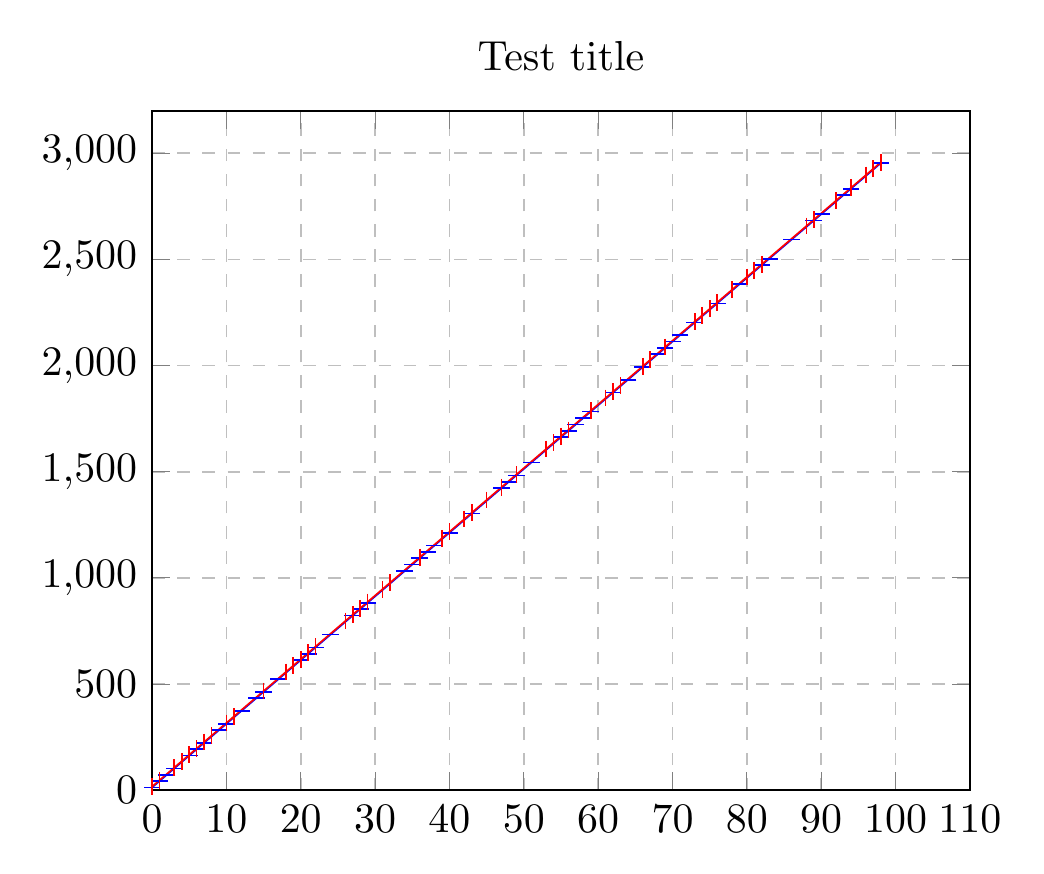
\begin{tikzpicture}[scale=\textwidth/8cm,]
	\begin{axis}[
	title={Test title},
	%xlabel={x label},
	%ylabel={y label},
	xmin=0, xmax=110,
	ymin=0, ymax=3200,
	xtick={0,10,20,30,40,50,60,70,80,90,100,110},
	ytick={0,500,1000,1500,2000,2500,3000},
	legend pos=north west,
	ymajorgrids=true,
	xmajorgrids=true,
	grid style=dashed,
	]
	
	\addplot[
	color=blue,
	%dotted,
	mark=-,
	%mark options={solid},
	%smooth
	%%mark=dot,
	]
	coordinates {
		(000,13)
		(001,43)
		(002,73)
		(003,103)
		(005,163)
		(006,193)
		(007,223)
		(009,283)
		(010,313)
		(012,373)
		(014,433)
		(015,463)
		(017,523)
		(020,613)
		(021,643)
		(022,673)
		(024,733)
		(027,823)
		(028,853)
		(029,883)
		(034,1033)
		(035,1063)
		(036,1093)
		(037,1123)
		(038,1153)
		(040,1213)
		(043,1303)
		(047,1423)
		(048,1453)
		(049,1483)
		(051,1543)
		(055,1663)
		(056,1693)
		(057,1723)
		(058,1753)
		(059,1783)
		(062,1873)
		(064,1933)
		(066,1993)
		(068,2053)
		(069,2083)
		(070,2113)
		(071,2143)
		(073,2203)
		(076,2293)
		(079,2383)
		(082,2473)
		(083,2503)
		(086,2593)
		(089,2683)
		(090,2713)
		(093,2803)
		(094,2833)
		(098,2953)
	};
	\addplot[
	color=red,
	%dotted,
	mark=|,
	%mark options={solid},
	%smooth
	%%mark=dot,
	]
	coordinates {
		(000,17)
		(001,47)
		(003,107)
		(004,137)
		(005,167)
		(006,197)
		(007,227)
		(008,257)
		(010,317)
		(011,347)
		(015,467)
		(018,557)
		(019,587)
		(020,617)
		(021,647)
		(022,677)
		(026,797)
		(027,827)
		(028,857)
		(029,887)
		(031,947)
		(032,977)
		(036,1097)
		(039,1187)
		(040,1217)
		(042,1277)
		(043,1307)
		(045,1367)
		(047,1427)
		(049,1487)
		(053,1607)
		(054,1637)
		(055,1667)
		(056,1697)
		(059,1787)
		(061,1847)
		(062,1877)
		(063,1907)
		(066,1997)
		(067,2027)
		(069,2087)
		(073,2207)
		(074,2237)
		(075,2267)
		(076,2297)
		(078,2357)
		(080,2417)
		(081,2447)
		(082,2477)
		(088,2657)
		(089,2687)
		(092,2777)
		(094,2837)
		(096,2897)
		(097,2927)
		(098,2957)
	};
	%\legend{CuSO$_4\cdot$5H$_2$O}
	\end{axis}
	\end{tikzpicture}
\end{center}

\pagebreak



\end{document}
